\chapter{Hasil Penelitian dan Pembahasan}


\section{Contoh Pembuatan Tabel}

Tapi kenyataan bagaimanapun juga harus diakui, bahwa mekanika Newton yang disokong oleh transformasi Galileo mengalami konflik dengan persamaan Maxwell. 

\begin{table}[h]
\centering
\caption{Judul tabel diletakkan di atas berbeda dengan caption untuk gambar}
\label{tab:tabelpertama}
\begin{tabular}{|l|l|l|}
\hline
saya & dia & kamu \\
\hline
saya & dia & kamu \\
saya & dia & kamu \\
saya & dia & kamu \\
\hline
\end{tabular}

\end{table}

\section{Contoh Menampilkan Gambar}
Sebagai salah satu upaya yang terbilang spektakuler untuk mendamaikan konflik antara mekanika Newton dan persamaan Maxwell dilakukan oleh Michelson dan Morley melalui serangkaian percobaan yang dilakukan dalam tahun 1887 dengan hipotesa bahwa ether itu ada. Namun Michelson-Morley pada akhirnya harus menerima kenyataan bahwa percobaannya menunjukkan bahwa ether tidak ada. Siapa sangka bahwa jalan keluar dari konflik antara mekanika Newton dan Persamaan Maxwell adalah usulan Einstein tersebut yang kini dikenal sebagai teori relativitas khusus.

\begin{figure}[h]
\centering
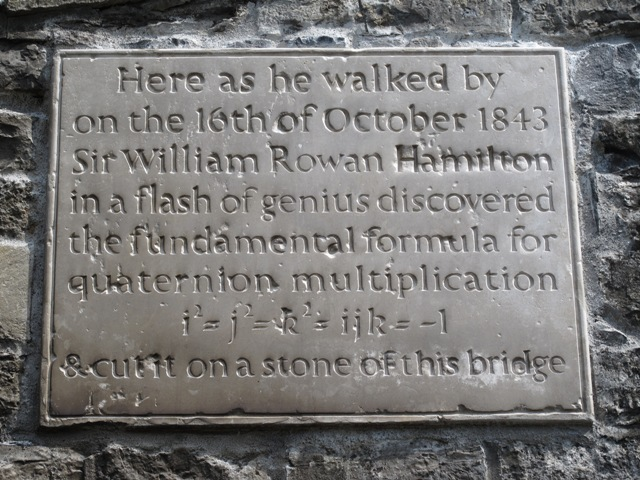
\includegraphics[scale=0.8]{gambarcontoh.jpg}
\caption{Gambar contoh pertama}
\label{gbr:gambarpertama}
\end{figure}

Sebagai salah satu upaya yang terbilang spektakuler untuk mendamaikan konflik antara mekanika Newton dan persamaan Maxwell dilakukan oleh Michelson dan Morley melalui serangkaian percobaan yang dilakukan dalam tahun 1887 dengan hipotesa bahwa ether itu ada. 

\section{Contoh merujuk ke tabel dan gambar}

Namun Michelson-Morley pada akhirnya harus menerima kenyataan bahwa percobaannya menunjukkan bahwa ether tidak ada. Siapa sangka bahwa jalan keluar dari konflik antara mekanika Newton dan Persamaan Maxwell adalah usulan Einstein tersebut yang kini dikenal sebagai teori relativitas khusus. 

Berdasarkan tabel \ref{tab:tabelpertama} dan gambar \ref{gbr:gambarpertama}, maka sebaiknya begitu.